% !TEX TS-program = xelatex
% !TEX encoding = UTF-8 Unicode
% !Mode:: "TeX:UTF-8"

\documentclass{resume}
\usepackage{zh_CN-Adobefonts_external} % Simplified Chinese Support using external fonts (./fonts/zh_CN-Adobe/)
% \usepackage{NotoSansSC_external}
% \usepackage{NotoSerifCJKsc_external}
% \usepackage{zh_CN-Adobefonts_internal} % Simplified Chinese Support using system fonts
\usepackage{linespacing_fix} % disable extra space before next section
\usepackage{cite}
\usepackage{graphicx}
\usepackage{tikz}

\begin{document}

\pagenumbering{gobble} % suppress displaying page number

\name{朱奎\quad James}

\basicInfo{
  \hspace{-2.5cm}
  \email{zhukui.1998@qq.com} \textperiodcentered\ 
  \phone{(+86) 131-2671-6166}
}
\basicInfo{
  \hspace{-2.5cm}
  \faHome 山东 潍坊\:\textperiodcentered\:\
  \faLaptop 后端开发、数据工程\:\textperiodcentered\:\
  \faMars 男
}
\begin{tikzpicture}[remember picture, overlay]

  \node [anchor=north east, outer sep=3.3cm,  outer ysep=1.2cm]  
  at (current page.north east) 
     {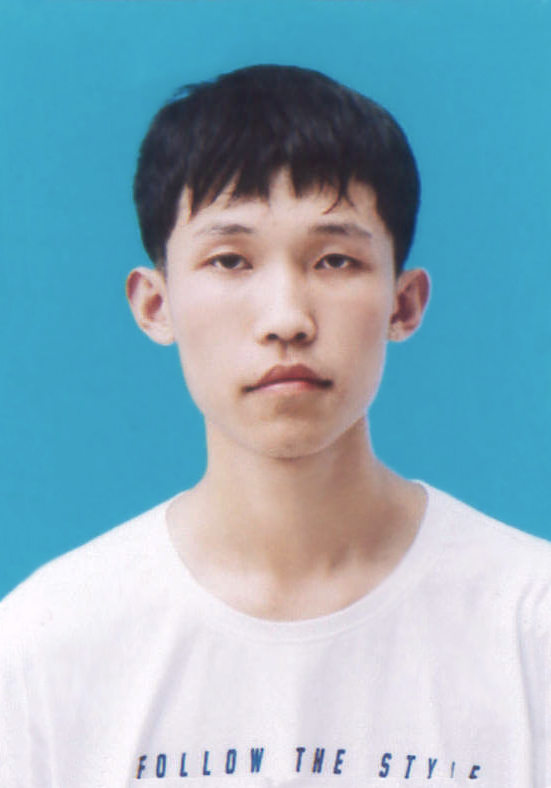
\includegraphics[width=2.3cm]{证件照.jpg}};
\end{tikzpicture}

  % \linkedin[billryan8]{https://www.linkedin.com/in/billryan8}}
  \section{\faGraduationCap\ 教育背景}
  \datedsubsection{\textbf{中国科学院大学},计算机软件与理论}{2021.9 - 预计2024.6毕业}
  \begin{itemize}
    \item \textit{学术硕士在读(保研)}
    \item \textbf{GPA:} 3.5 / 4.0\space \space \textbf{排名:} 4 /  63 (前10\%)
  \end{itemize}
  \datedsubsection{\textbf{河南科技大学},计算机科学与技术}{2017.9 - 2021.6}
  \begin{itemize}
    \item \textit{本科}
    \item \textbf{GPA:} 4.5 / 5.0\space \space \textbf{排名:} 3 / 144 (前3\%)
  \end{itemize}

  \section{\faUsers\ 实习经历}

  \datedsubsection{\textbf{阿里巴巴(中国)集团控股有限公司}}{2023年6月 -- 2023年9月}
  \role{后端开发实习生}{飞猪·住宿行业基础平台--国际EBK·商品}
  \textbf{国际EBK商品直连系统} 
   \begin{spacing}{1.2} 
  国内酒店商品EBK直连系统对于国际化能力、多币种结算、税费合规、\textbf{复杂商家类型和账号体系}权限体系等海外业务场景的支持不足,
  因此建立新的国际EBK直连系统,负责Java后端开发工作。

  \begin{itemize}
    \item 负责国际EBK直连系统的账号和权限模块开发,主要负责用户账号鉴权、联系人消息通知等模块的开发,通过主子账号、functionBit、角色授权等设计,实现了用户账号的\textbf{权限分配、鉴权、登录、子账号创建}以及\textbf{基于MetaQ}消息中间件实现了联系人的消息通知等功能。
    % \item 了解国际酒店EBK直连平台中营销能力设计,包括价库管理、价格联动、酒店促销、酒店优惠券等功能。
    \item 了解国际酒店EBK直连平台中\textbf{营销能力}设计和\textbf{供应商数据中心MOS}需求。MOS为国际EBK提供经营能力,帮助供应商感知N漏斗全过程,能够通过数据快速定位并提升整体酒店/房型匹配率,通过价格数据雷达的呈现,帮助供应商确定价格在飞猪侧的竞争力,辅助其进行调价。
  \end{itemize}
  \end{spacing}

  \datedsubsection{\textbf{微软(亚洲)互联网工程院}}{2022年11月 -- 2023年5月}
  \role{数据/软件开发实习生(Data/Software Develop Engineer Intern)}{STCA Beijing Bing}

  1. \textbf{Microsoft Creator Copilot (微软内容创作者助手)} 
  \begin{spacing}{1.2} 
  基于Bing搜索引擎和ChatGPT模型的\textbf{AIGC自动创作工具},提供段落实时改写、热搜话题新闻生成以及自动配图等功能。
  主要负责\textbf{后端系统}开发。
  \begin{itemize}
    % ReAct框架将对话系统的任务分解为两种类型的动作:推理动作(Reasoning Actions)和搜索动作(Search Actions)。推理动作是指LLM根据当前的对话状态和用户输入,生成一个或多个候选的回答或询问。搜索动作是指LLM根据当前的对话状态和用户输入,生成一个或多个候选的搜索查询,并利用搜索引擎获取相关的搜索结果。
    \item 采用\textbf{代理模式}设计\textbf{代理层}和\textbf{业务层}。代理层负责与\textbf{搜索引擎和LLM模型服务接口进行交互},实现搜索、模型的调用和结果返回。业务层负责处理用户请求和响应,实现写作工具的核心功能。为了提高框架的性能和生成质量,我在代理层采用了\textbf{接口响应优化、HTTP连接池、线程池、Redis缓存}等技术,有效地提升了并发请求的吞吐量和响应速度。
    \item Prompt工程:采用LLM ReAct(Reasoning and Acting)范式,结合\textbf{推理}动作和\textbf{搜索}动作功能使ChatGPT模型可以与Bing搜索引擎交互,获取\textbf{实时热搜话题}和\textbf{Bing搜索结果}作为知识库,克服了思维链推理中普遍存在的妄想和错误传播问题,并生成更合理的类人任务解决轨迹,提高大语言模型AI新闻创作的真实性和创造性。
  \end{itemize}
  2. \textbf{Bing用户增长数据工程 \& 搜索平台工具}
  \begin{itemize}
    \item 负责Bing Search中\textbf{用户搜索相关的数据开发和数据分析},使用微软Cosmos数据平台Scope语言(类Hive SQL)对Bing搜索引擎实时日志数据进行ETL,产出关于增长、日活、群体、地域、热搜话题等图表,结合可视化用户增长平台进行监控,并进行分析;改进本土化搜索的业务策略和功能、分析修复线上bug,提高DAU、DSQ等用户增长指标,并通过ABTest平台进行分析,最终提升了搜索用户体验。
    \item 维护\textbf{Bing Search}的平台工具,负责\textbf{Bing中国区首页新闻热点数据的更新}业务功能。首先ETL产出的热搜数据实时入库,通过调度框架执行Azure function实现从KV存储中读取热搜数据进行提取、加工、转换。完善Bing HotSearch热搜、Bing新标签页股票指数更新等功能的链路。
  \end{itemize}
\end{spacing}
 
  \datedsubsection{\textbf{上海哔哩哔哩科技有限公司}}{2022年6月 -- 2022年9月}
  \role{数据平台Java后端开发实习生}{bilibili 数据平台部 Berserker}
  \textbf{B站大数据平台·平台工具·元数据}
\begin{spacing}{1.2} 
  % Berserker是提供数据的存储、查询、数据开发、数据质量分析、分布式调度的大数据平台。
  实习中负责工具侧\textbf{元数据、数据运营、数据管理}等方向,专注\textbf{元数据采集、治理工具}等功能的研发。

  \begin{itemize}
    \item 设计了Hive MetaStore中\textbf{分区信息数据的解耦方案}。通过\textbf{全量拷贝、Binlog增量变更、数据一致性检测、分布式调度同步}的方法落入\textbf{TiDB}的方案加速查询,优化了Hive表分区信息查询速度和资源占用,\textbf{接口性能提升60\%}
    \item 在部门降本增效计划中,参与了无效数据表集中下线的功能设计,为业务提供打标,批量定时删除并在删除后及时告知表所有人的功能,通过\textbf{分布式定时调度框架}设计实现了高效的数据表安全删除逻辑功能
    % \item 为了提高数据访问的性能,需要区分\textbf{冷热数据}。同时,为了支持各类数据应用和数据治理的需求,需要提供表使用热度的统计和查询功能,在数据库层面统计各个表的使用情况,设计了覆盖全、数据准、粒度细的\textbf{表使用热度}功能服务,为各类数据应用和数据治理提供支持。
  \end{itemize}
  \end{spacing} 
    % 在大数据场景下,数据量庞大,存储成本高,缓存利用率低。为了提高数据访问的效率和性能,需要区分冷热数据,将热数据缓存到高速存储介质上,将冷数据迁移到低成本存储介质上。同时,为了支持各类数据应用和数据治理的需求,需要提供表使用热度的统计和查询功能。

    % 业务结果:通过表使用热度功能服务,可以实现以下目标:
    
    % 节约整体的存储成本,降低冷数据的占用空间。
    % 提高缓存利用效率,加速热数据的访问速度。
    % 支持各类数据应用和数据治理的分析和决策,如优化表结构、调整分区策略、制定归档策略等。
    %     1. 数据库层面的数据统计
% 首先,您需要在数据库层面统计各个表的使用情况。将各类数据的使用情况包括应用访问次数、访问时长、操作类型、查询条件等信息统计到数据库表中。这个数据库表可以设计成包含数据表ID、表名、应用名称、数据访问次数、访问时长、最近访问时间等字段。

% 2. 统计分析
% 对于每张表所记录的访问信息,您需要进行统计分析,并对结果进行存储。您可以使用spark等大数据框架处理这些访问数据,包括按访问次数或访问时长排序,统计每个应用对每个表的访问情况等。具体操作可以根据业务需求和数据量大小进行选择。

% 3. 热度服务接口的实现
% 将前两个步骤统计和分析的结果封装成热度服务接口,提供给各类数据应用和数据治理使用。该接口可以设计为Restful风格,支持各种访问方式,比如查询某个数据表的热度,查询某个应用对某张数据表的访问情况等。接口返回内容可以根据业务需求进行设计,比如返回数据表的名字、使用次数和使用时长等维度的指标。

% 4. 热度展示信息的呈现
% 最后,您需要将热度服务接口的结果进行呈现。可以在数据平台的首页、数据目录、应用界面等位置展示表的热度信息、趋势图、排行榜等。同时也可以通过热度服务提供给数据治理使用,比如对使用次数较少的表进行删除、对使用靠前的表进行备份、对数据质量较差的表进行整理等。

% 总结起来,通过对数据库层面的数据统计、分析和封装成服务接口,实现数据热度的收集和展示,这有助于提升大数据平台的数据应用价值,优化数据治理等业务操作,从而进一步提高数据质量和增强数据资产价值。



  % \section{\faUsers\ 项目经历}
  % \datedsubsection{\textbf{用于列车售票的可线性化并发数据结构}}{2021年9月 -- 2021年12月}
  % \role{个人项目}{中国科学院大学《并发数据结构与多核编程》,林惠民院士}
  % \begin{spacing}{1.2}
  %   使用Java语言设计并完成了一个\textbf{用于列车售票的可线性化并发数据结构}
  %   \begin{itemize} 
  %     \item 支持查票、购票、退票等操作,同时保证每个操作都能\textbf{线性化}地执行,即在并发环境下,每个操作都能按照某个全局顺序执行,不会出现不一致或冲突的情况。 
  %     \item 采用乘车区间\textbf{二进制编码运算}的算法,将每个区间用一个二进制位表示,从而将锁的粒度从区间级别降低到位级别,大大减少了锁的竞争和开销。同时,基于\textbf{CAS原语}(比较并交换),实现了\textbf{lock-free}(无锁)的并发方案,避免了死锁、饥饿等问题,提高了并发效率。 
  %     \item 引入余票表缓存,在购票、退票后多线程异步刷新余票表,使得查票操作可以直接从缓存中读取数据,提高了查询速度;同时通过随机占座等负载均衡的优化,使得不同线程尽量访问不同的资源,避免了资源竞争,提高了并发性能。 
  %     \item 按照70\%查票、20\%购票、10\%退票的概率进行压力测试,利用吞吐量、操作时延等性能评价指标,对算法性能进行评估,最终性能评测分数排名达到所有方案的\textbf{前5\%}。并且使用可线性化验证工具对并发数据结构进行可线性化分析验证,证明了算法的正确性。
  %     \item 使用日志系统进行容灾处理,即每次执行操作时都会记录操作的类型、参数、结果等信息到一个日志文件中。这样可以保证在断电后可以根据日志文件重放操作,并且恢复到最新的状态。
  %    \end{itemize} 
  % \end{spacing}


  \section{\faUsers\ 个人项目} 
  \datedsubsection{\textbf{用于列车售票的可线性化并发数据结构}}{2021年9月 - 2021年12月} 
  \role{课程设计}{中国科学院大学《并发数据结构与多核编程》,林惠民} 
 在本项目中,使用Java语言设计并实现了一个\textbf{基于lock-free算法的高效列车售票系统},该系统支持查票、购票、退票等操作,并能在并发环境下保证高性能运行。
 \begin{spacing}{1.2}
    \begin{itemize} 
      \item 利用乘车区间\textbf{二进制编码运算}的技术,将每个区间用一个二进制位表示,从而将锁的粒度从区间级别降低,大大减少了锁的竞争和开销。 
      \item 基于\textbf{CAS原语}(比较并交换),实现了\textbf{lock-free}(无锁)的并发方案,避免了死锁、饥饿等问题,提高了并发效率。 
      \item 引入余票表\textbf{缓存},在购票、退票后子线程异步刷新余票表,使得查票操作可以直接从缓存中读取数据,提高了查询速度;通过随机占座等\textbf{负载均衡}的优化,使得不同线程尽量访问不同的资源,避免了资源竞争,提高了并发性能。 
      \item 按照70\%查票、20\%购票、10\%退票的概率进行压力测试,利用\textbf{吞吐量、操作时延}等性能评价指标,对算法性能进行评估,最终性能评测分数排名达到所有方案的\textbf{前5\%}。并且使用可线性化验证工具对并发数据结构进行可线性化分析验证,证明了算法的正确性。 
    \end{itemize} 
  \end{spacing}


% \datedsubsection{\textbf{中铁隧道局集团有限公司}}{2019 年9月 -- 2019 年 12 月}
% \role{移动端负责人}{中铁隧道局机况检测系统}
% \begin{spacing}{1.2}
% 移动端设备检测模块Android项目负责人,协调后端开发
% \begin{itemize}
%   \item 实现了隧道局盾构机机况检测App,设计了\textbf{图像压缩、数据可靠传输、系统安全性保障}的方案
%   \item 参与了基于SpringBoot框架的中铁隧道局管理系统后端开发,负责\textbf{用户权限管理}和\textbf{安全性校验}的设计。
%   \item 负责项目部署和企业工作人员对接,此项目\textbf{已上线}应用于中铁隧道局集团有限公司日常的盾构机机况检测工作中。
%   \item 涉及技术:Java、SpringBoot、Android
% \end{itemize}
% \end{spacing}

% Reference Test
%\datedsubsection{\textbf{Paper Title\cite{zaharia2012resilient}}}{May. 2015}
%An xxx optimized for xxx\cite{verma2015large}
%\begin{itemize}
%  \item main contribution
%\end{itemize}

\section{\faHeartO\ 获奖情况}
\begin{itemize}[parsep=0.5ex]
  \item 中国科学院大学三好学生
  \item 国家励志奖学金
  \item 中国科学院大学计算机科学与技术学院优秀学生
  \item 全国大学生数学建模竞赛省二等奖
  \item 全国大学生数学竞赛三等奖
\end{itemize}

\section{\faCogs\ 爱好与技能}
\begin{itemize}[parsep=0.5ex]
  \item 英语 :		   CET 4 566、CET 6 479
  \item 爱好 :		   乒乓球、羽毛球、游戏(飞猪王者荣耀联赛总冠军)
  \item 文档 :		   Markdown、\LaTeX
\end{itemize}


% \section{\faInfo\ 其他}
% % increase linespacing [parsep=0.5ex]
% \begin{itemize}[parsep=0.5ex]
%   \item GitHub: https://github.com/username
%   \item 语言: 英语 - 熟练(TOEFL xxx)
% \end{itemize}

%% Reference
%\newpage
%\bibliographystyle{IEEETran}
%\bibliography{mycite}
\end{document}
